\part{Anhang}

\section*{Prozentuale Speichergröße abhängig zur Kompressionsqualität}
\begin{itemize}
    \item Durchschn. Gr. [\%] = 1.7753, Var (0.0116), Std (0.1079), Kompression 5
    \item Durchschn. Gr. [\%] = 2.2008, Var (0.0454), Std (0.2131), Kompression 10
    \item Durchschn. Gr. [\%] = 2.5956, Var (0.0925), Std (0.3042), Kompression 15
    \item Durchschn. Gr. [\%] = 2.9598, Var (0.1483), Std (0.3852), Kompression 20
    \item Durchschn. Gr. [\%] = 3.3149, Var (0.2125), Std (0.4609), Kompression 25
    \item Durchschn. Gr. [\%] = 3.6475, Var (0.2803), Std (0.5294), Kompression 30
    \item Durchschn. Gr. [\%] = 4.2521, Var (0.4210), Std (0.6489), Kompression 40
    \item Durchschn. Gr. [\%] = 4.8640, Var (0.5814), Std (0.7625), Kompression 50
    \item Durchschn. Gr. [\%] = 5.5362, Var (0.7793), Std (0.8828), Kompression 60
    \item Durchschn. Gr. [\%] = 6.6223, Var (1.1183), Std (1.0575), Kompression 70
    \item Durchschn. Gr. [\%] = 7.3122, Var (1.3500), Std (1.1619), Kompression 75
    \item Durchschn. Gr. [\%] = 10.0661, Var (2.3375), Std (1.5289), Kompression 85
    \item Durchschn. Gr. [\%] = 13.0879, Var (3.5185), Std (1.8758), Kompression 90
    \item Durchschn. Gr. [\%] = 20.1317, Var (6.6612), Std (2.5809), Kompression 95
    \item Durchschn. Gr. [\%] = 49.6575, Var (19.2566), Std (4.3882), Kompression 100
\end{itemize}


\newpage
\section*{Kompressionsfaktor abhängig zur Kompressionsqualität}

\begin{itemize}
    \item Faktor = 56.3271, Var (11.7193), Std (3.4233), Kompression 5
    \item Faktor = 45.4375, Var (19.3515), Std (4.3990), Kompression 10
    \item Faktor = 38.5274, Var (20.3912), Std (4.5157), Kompression 15
    \item Faktor = 33.7861, Var (19.3303), Std (4.3966), Kompression 20
    \item Faktor = 30.1667, Var (17.5956), Std (4.1947), Kompression 25
    \item Faktor = 27.4159, Var (15.8330), Std (3.9791), Kompression 30
    \item Faktor = 23.5180, Var (12.8794), Std (3.5888), Kompression 40
    \item Faktor = 20.5591, Var (10.3865), Std (3.2228), Kompression 50
    \item Faktor = 18.0628, Var (8.2953), Std (2.8801), Kompression 60
    \item Faktor = 15.1006, Var (5.8148), Std (2.4114), Kompression 70
    \item Faktor = 13.6758, Var (4.7222), Std (2.1731), Kompression 75
    \item Faktor = 9.9343, Var (2.2767), Std (1.5089), Kompression 85
    \item Faktor = 7.6407, Var (1.1992), Std (1.0951), Kompression 90
    \item Faktor = 4.9673, Var (0.4055), Std (0.6368), Kompression 95
    \item Faktor = 2.0138, Var (0.0317), Std (0.1780), Kompression 100
\end{itemize}


\newpage
\section*{SSIM, PSNR, MSE Werte}
        \begin{table}[h!]
\centering
\begin{tabular}{|c|c|c|c|}
\hline
\textbf{Kompression} & \textbf{SSIM} & \textbf{PSNR} & \textbf{MSE} \\ \hline
5                    & 0.6345        & 75.7594       & 0.001747     \\ \hline
10                   & 0.8007        & 79.1075       & 0.000807     \\ \hline
15                   & 0.8876        & 81.4212       & 0.000477     \\ \hline
20                   & 0.9229        & 83.0211       & 0.000333     \\ \hline
25                   & 0.9359        & 83.9889       & 0.000268     \\ \hline
30                   & 0.9412        & 84.5488       & 0.000236     \\ \hline
40                   & 0.9533        & 85.6218       & 0.000185     \\ \hline
50                   & 0.9613        & 86.4335       & 0.000154     \\ \hline
60                   & 0.9646        & 86.9647       & 0.000137     \\ \hline
70                   & 0.9697        & 87.7416       & 0.000115     \\ \hline
75                   & 0.9730        & 88.2414       & 0.000103     \\ \hline
85                   & 0.9779        & 89.3331       & 0.000080     \\ \hline
90                   & 0.9811        & 90.1780       & 0.000065     \\ \hline
95                   & 0.9853        & 91.6023       & 0.000047     \\ \hline
100                  & 0.9938        & 95.7158       & 0.000018     \\ \hline
vq-f16               & 0.8769        & 76.5315       & 0.001559     \\ \hline
vq-f8-n256           & 0.9020        & 78.4603       & 0.000987     \\ \hline
\end{tabular}
\caption{Übersicht der Kompressionswerte mit SSIM, PSNR und MSE.}
\label{tab:compression}
\end{table}

\newpage
\section*{Precisiom, Recall, F1-Score Werte}
\begin{table}[h!]
\centering
\begin{tabular}{|c|c|c|c|}
\hline
\textbf{Kompression} & \textbf{Precision} & \textbf{Recall} & \textbf{F1} \\ \hline
5                    & 0.7965             & 0.4856          & 0.6034      \\ \hline
10                   & 0.8543             & 0.6439          & 0.7343      \\ \hline
15                   & 0.9144             & 0.7710          & 0.8366      \\ \hline
20                   & 0.9383             & 0.8372          & 0.8849      \\ \hline
25                   & 0.9488             & 0.8642          & 0.9045      \\ \hline
30                   & 0.9553             & 0.8774          & 0.9147      \\ \hline
40                   & 0.9611             & 0.8996          & 0.9293      \\ \hline
50                   & 0.9652             & 0.9127          & 0.9382      \\ \hline
60                   & 0.9677             & 0.9185          & 0.9424      \\ \hline
70                   & 0.9708             & 0.9274          & 0.9486      \\ \hline
75                   & 0.9724             & 0.9343          & 0.9530      \\ \hline
85                   & 0.9750             & 0.9463          & 0.9604      \\ \hline
90                   & 0.9755             & 0.9530          & 0.9641      \\ \hline
95                   & 0.9777             & 0.9638          & 0.9707      \\ \hline
100                  & 0.9802             & 0.9749          & 0.9775      \\ \hline
vq-f16              & 0.9472             & 0.8019          & 0.8685      \\ \hline
vq-f8-n256         & 0.9515             & 0.8685          & 0.9081      \\ \hline
\end{tabular}
\caption{Übersicht der Kompressionswerte mit Precision, Recall und F1-Score.}
\label{tab:compression_metrics}
\end{table}

\newpage
    \section*{Durchschnittliche IoU-Werte und Statistiken}

\begin{itemize}
    \item Durchschn. IoU = 0.4467, Var (0.1901), Std (0.4360), Kompression 5
    \item Durchschn.  IoU = 0.5737, Var (0.1753), Std (0.4187), Kompression 10
    \item Durchschn.  IoU = 0.6772, Var (0.1461), Std (0.3822), Kompression 15
    \item Durchschn.  IoU = 0.7514, Var (0.1176), Std (0.3429), Kompression 20
    \item Durchschn.  IoU = 0.7916, Var (0.1007), Std (0.3173), Kompression 25
    \item Durchschn.  IoU = 0.8135, Var (0.0913), Std (0.3021), Kompression 30
    \item Durchschn.  IoU = 0.8439, Var (0.0769), Std (0.2774), Kompression 40
    \item Durchschn.  IoU = 0.8648, Var (0.0667), Std (0.2584), Kompression 50
    \item Durchschn.  IoU = 0.8757, Var (0.0626), Std (0.2502), Kompression 60
    \item Durchschn.  IoU = 0.8901, Var (0.0550), Std (0.2345), Kompression 70
    \item Durchschn.  IoU = 0.9004, Var (0.0497), Std (0.2229), Kompression 75
    \item Durchschn.  IoU = 0.9193, Var (0.0397), Std (0.1993), Kompression 85
    \item Durchschn.  IoU = 0.9293, Var (0.0346), Std (0.1859), Kompression 90
    \item Durchschn.  IoU = 0.9442, Var (0.0263), Std (0.1621), Kompression 95
    \item Durchschn.  IoU = 0.9609, Var (0.0174), Std (0.1319), Kompression 100
    \item Durchschn.  IoU = 0.7951, Var (0.1002), Std (0.3165), Kompression vq-f8-f256
    \item Durchschn.  IoU = 0.7092, Var (0.1364), Std (0.3693), Kompression vq-f16
\end{itemize}

\part{Anhang}
\section*{Latente Darstellung des vq-f16-Modells (Aachen erstes Bild)}
     
            \begin{figure}[!htb]
                \centering
                \begin{minipage}[!htb]{0.47\textwidth}
                    \centering
                    \textbf{Kanal 1} % Überschrift für die erste Spalte
                \end{minipage}
                %
                \begin{minipage}[!htb]{0.47\textwidth}
                    \centering
                    \textbf{Kanal 2} % Überschrift für die zweite Spalte
                \end{minipage}
    
                \begin{minipage}[!htb]{0.48\textwidth}
                    \centering
                    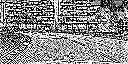
\includegraphics[width=\textwidth]{pictures/vq-f16_latent_channel_1.png}    
                \end{minipage}
                %
                \begin{minipage}[!htb]{0.48\textwidth}
                    \centering
                    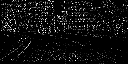
\includegraphics[width=\textwidth]{pictures/vq-f16_latent_channel_2.png}
                \end{minipage}
            \end{figure}
            \begin{figure}[!htb]
                \centering
                \begin{minipage}[!htb]{0.47\textwidth}
                    \centering
                    \textbf{Kanal 3} % Überschrift für die erste Spalte
                \end{minipage}
                %
                \begin{minipage}[!htb]{0.47\textwidth}
                    \centering
                    \textbf{Kanal 4} % Überschrift für die zweite Spalte
                \end{minipage}
    
                \begin{minipage}[!htb]{0.48\textwidth}
                    \centering
                    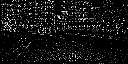
\includegraphics[width=\textwidth]{pictures/vq-f16_latent_channel_3.png}    
                \end{minipage}
                %
                \begin{minipage}[!htb]{0.48\textwidth}
                    \centering
                    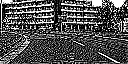
\includegraphics[width=\textwidth]{pictures/vq-f16_latent_channel_4.png}
                \end{minipage}
            \end{figure}
            \begin{figure}[!htb]
                \centering
                \begin{minipage}[!htb]{0.47\textwidth}
                    \centering
                    \textbf{Kanal 5} % Überschrift für die erste Spalte
                \end{minipage}
                %
                \begin{minipage}[!htb]{0.47\textwidth}
                    \centering
                    \textbf{Kanal 6} % Überschrift für die zweite Spalte
                \end{minipage}
    
                \begin{minipage}[!htb]{0.48\textwidth}
                    \centering
                    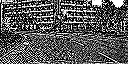
\includegraphics[width=\textwidth]{pictures/vq-f16_latent_channel_5.png}    
                \end{minipage}
                %
                \begin{minipage}[!htb]{0.48\textwidth}
                    \centering
                    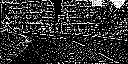
\includegraphics[width=\textwidth]{pictures/vq-f16_latent_channel_6.png}
                \end{minipage}
            \end{figure}
            \begin{figure}[!htb]
                \centering
                \begin{minipage}[!htb]{0.47\textwidth}
                    \centering
                    \textbf{Kanal 7} % Überschrift für die erste Spalte
                \end{minipage}
                %
                \begin{minipage}[!htb]{0.47\textwidth}
                    \centering
                    \textbf{Kanal 8} % Überschrift für die zweite Spalte
                \end{minipage}
    
                \begin{minipage}[!htb]{0.48\textwidth}
                    \centering
                    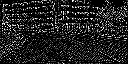
\includegraphics[width=\textwidth]{pictures/vq-f16_latent_channel_7.png}    
                \end{minipage}
                %
                \begin{minipage}[!htb]{0.48\textwidth}
                    \centering
                    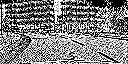
\includegraphics[width=\textwidth]{pictures/vq-f16_latent_channel_8.png}
                \end{minipage}
            \end{figure}
            
\newpage
\section*{Latente Darstellung des vq-f8-n256-Modells (Aachen erstes Bild)}
     
            \begin{figure}[!htb]
                \centering
                \begin{minipage}[!htb]{0.47\textwidth}
                    \centering
                    \textbf{Kanal 1} % Überschrift für die erste Spalte
                \end{minipage}
                %
                \begin{minipage}[!htb]{0.47\textwidth}
                    \centering
                    \textbf{Kanal 2} % Überschrift für die zweite Spalte
                \end{minipage}
    
                \begin{minipage}[!htb]{0.48\textwidth}
                    \centering
                    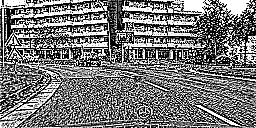
\includegraphics[width=\textwidth]{pictures/vq-f8-n256_latent_channel_1.png}    
                \end{minipage}
                %
                \begin{minipage}[!htb]{0.48\textwidth}
                    \centering
                    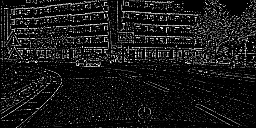
\includegraphics[width=\textwidth]{pictures/vq-f8-n256_latent_channel_2.png}
                \end{minipage}
            \end{figure}
            \begin{figure}[!htb]
                \centering
                \begin{minipage}[!htb]{0.47\textwidth}
                    \centering
                    \textbf{Kanal 3} % Überschrift für die erste Spalte
                \end{minipage}
                %
                \begin{minipage}[!htb]{0.47\textwidth}
                    \centering
                    \textbf{Kanal 4} % Überschrift für die zweite Spalte
                \end{minipage}
    
                \begin{minipage}[!htb]{0.48\textwidth}
                    \centering
                    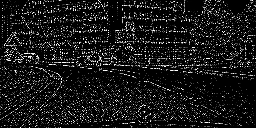
\includegraphics[width=\textwidth]{pictures/vq-f8-n256_latent_channel_3.png}    
                \end{minipage}
                %
                \begin{minipage}[!htb]{0.48\textwidth}
                    \centering
                    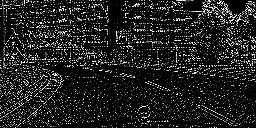
\includegraphics[width=\textwidth]{pictures/vq-f8-n256_latent_channel_4.png}
                \end{minipage}
            \end{figure}
    